% tikzpic.tex
\documentclass[crop]{standalone}% 'crop' is the default for v1.0, before it was 'preview'
\usepackage{testpackage}
\setromanfont{Fira Sans}
\setmainfont{Fira Sans}
\everymath\expandafter{\the\everymath\rm}
\everydisplay\expandafter{\the\everydisplay\rm}
%\usetikzlibrary{...}% tikz package already loaded by 'tikz' option
\usepackage{tikz,pgfplots}
\usepackage{array}




\begin{document}
	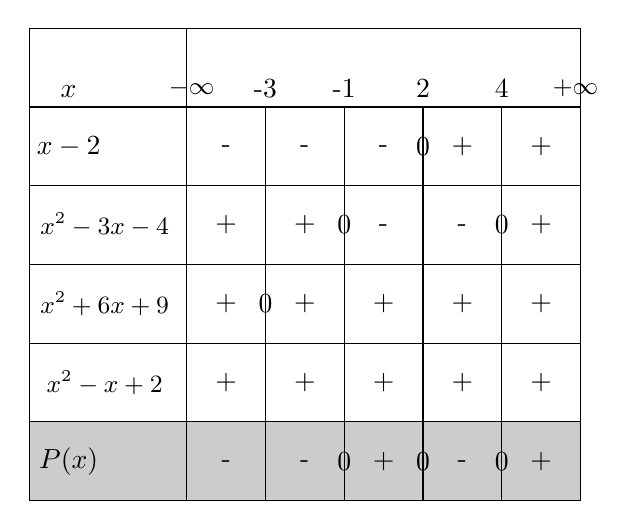
\begin{tikzpicture}
	\filldraw[fill=black!20, draw=black!10](0,0) rectangle (7,1);
	\draw (0,0) rectangle (7,6);
	\draw (2,0)--(2,6);
	\draw(0,1)--(7,1);
	\draw(0,2)--(7,2);
	\draw(0,3)--(7,3);
	\draw(0,4)--(7,4);
	\draw(0,5)--(7,5);
	\draw(3,0)--(3,5) node[above]{-3};
	\draw(4,0)--(4,5)node[above]{-1};
	\draw(5,0)--(5,5)node[above]{2};
	\draw(6,0)--(6,5)node[above]{4};
	\node[above right,xshift=-10] at (2,5){\small$-\infty$};
	\node[above left,xshift=10] at (7,5){\small$+\infty$};
	\node at (0.5,4.5){$x-2$};\node at (2.5,4.5){-};\node at (3.5,4.5){-};\node at (4.5,4.5){-};\node at (5.5,4.5){+};\node at (6.5,4.5){+};\node at (5,4.5){0};
	\node [xshift=13]at (0.5,3.5){\small$x^2-3x-4$};\node at (2.5,3.5){+};\node at (3.5,3.5){+};\node at (4.5,3.5){-};\node at (5.5,3.5){-};\node at (6.5,3.5){+};\node at (4,3.5){0};\node at (6,3.5){0};
	\node  [xshift=13]at (0.5,2.5){\small$x^2+6x+9$};\node at (2.5,2.5){+};\node at (3.5,2.5){+};\node at (4.5,2.5){+};\node at (5.5,2.5){+};\node at (6.5,2.5){+};\node at (3,2.5){0};
	\node [xshift=13]at (0.5,1.5){\small$x^2-x+2$};\node at (2.5,1.5){+};\node at (3.5,1.5){+};\node at (4.5,1.5){+};\node at (5.5,1.5){+};\node at (6.5,1.5){+};
	\node at (0.5,0.5){$P(x)$};\node at (2.5,0.5){-};\node at (3.5,0.5){-};\node at (4.5,0.5){+};\node at (5.5,0.5){-};\node at (6.5,0.5){+};\node at (6,0.5){0};\node at (5,0.5){0};\node at (4,0.5){0};
	\node [above]at (0.5,5){$x$};
	\end{tikzpicture}
\end{document}